%!TEX root = ../../../thesis.tex

\section{The Scott-Single Interface Model}

  \begin{figure}
    \centering
    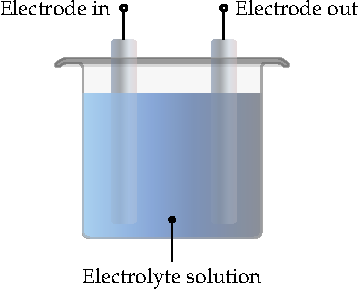
\includegraphics{content/pt2/07-InterfaceModel/graphics/electrode-electrolyte}
    \caption{\label{fig:electrode-electrolyte}Electrodes submerged in an electrolyte solution, such a system can be described by the Scott-Single Interface Model.}
  \end{figure}

  Jonathan Scott and Peter Single recently published an electrical model of an implantable electrode array in saline \cite{ScottSingle2013}.
  The intention of that model is to simulate what a medical implant device would see once implanted into a human spinal cavity.
  Because it uses a minimum number of parameters to generate the model and therefore simulate the system, it is compact.
  It is also general enough to use in any situation where electrodes are placed in an electrolyte solution, such as depicted in \cref{fig:electrode-electrolyte}.

  \begin{figure}
    \centering
    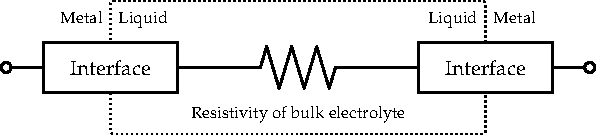
\includegraphics{content/pt2/07-InterfaceModel/graphics/simpleElectrodeElectrolyteModel}
    \caption{\label{fig:pt2-simpleElectrodeElectrolyteModel}Connection diagram of two interface models connected together by the resistivity of an electrolyte solution.}
  \end{figure}
  The model comes in two parts, the electrode interface and the resistivity of the electrolyte's bulk.
  \Cref{fig:pt2-simpleElectrodeElectrolyteModel} shows the general electrical configuration of such an electrode-electrolyte system.
  It shows that there are two interfaces per system, and that the liquid side of those two interfaces are joined electrically by the resistance of the electrolyte's bulk resistivity.
  The metal side of the interfaces is what the rest of the circuit would connect to, perhaps batteries and lights.


  % The model contains both the electrode-electrolyte interface and the resistivity of the electrolyte's bulk.

  % The interface model and its accompanying resistive mesh was developed specifically to calculate the impedance between the electrodes of an eight electrode array, such as is used in spinal cord stimulation.



  \subsection{The interface model}

    % \begin{figure}
    %   \centering
    %   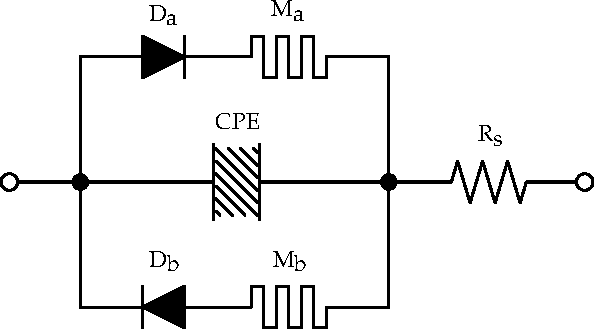
\includegraphics{content/pt2/07-InterfaceModel/graphics/interfaceSchematic}
    %   \caption{\label{fig:pt2-interfaceSchematic}Electrical schematic of the electrode-electrolyte interface}
    % \end{figure}

    The Scott-Single interface is modelled by the circuit shown in \cref{fig:pt2-interfaceSchematic}.
    Each of the components and their functions will be explained in the coming sections.
    It is important to realise that this model only represents a single interface between metal and electrolyte.
    By itself it is incapable of simulating any useful electrode/electrolyte system.
    For that, a minimum of two interfaces must be used - one as a cathode and one as an anode.
    Additionally, some model of the electrolyte resistivity needs to connect the two interfaces.


    \Cref{fig:pt2-simpleElectrodeElectrolyteModel} shows the smallest/simplest use of the interface model.
    This configuration represents two electrodes placed in an electrolyte solution.
    It allows simulation of impedance between those electrodes and can be connected to other electronic circuits.
    A model like this is only valid for a two electrode system.
    Because the electrode array in our application has eight electrodes, the model is more complex.
    In full, that model will have eight electrode interfaces and a resistor network connecting each interface.

    \subsubsection{Polar effects: Constant phase element}
      At the centre of the model is the constant phase element, or CPE.
      This element behaves like a capacitor, except for the fact that its impedance magnitude

    \subsubsection{Surface reactions: diodes}
    \subsubsection{Species depletion: memristors}

  \subsection{Inter-electrode resistivity}
    \begin{figure}
      \centering
      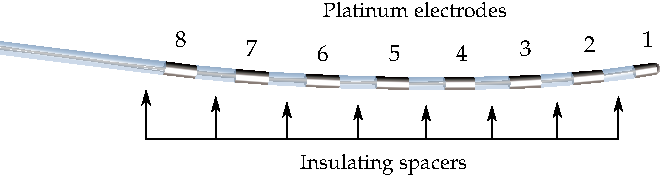
\includegraphics{content/pt2/07-InterfaceModel/graphics/StJudeOctrodeDiagram}
      \caption{\label{fig:StJudeOctrode_Labelled}St. Jude Medical Octrode. An eight electrode array commonly used in spinal stimulation implants.}
    \end{figure}

  % \Cref{fig:StJudeOctrode_Labelled} is an illustration of the electrode array and the numbering scheme used to identify each electrode.
  % Each electrode on this array is made from platinum and is separated by an insulating spacer.
  % The array has eight platinum wires that run through the cable to each of the electrodes.
  % This electrode was used through the remainder of this thesis and is the electrode used by Saluda in medical trials of their stimulators.

  % \begin{figure}
  %   \centering
  %   \includegraphics{content/pt2/07-InterfaceModel/graphics/interfaceSchematic_noMemristive}
  %   \caption{\label{fig:pt2-interfaceSchematic_noMemristive}Electrical schematic of the electrode-electrolyte interface with the memristors omitted}
  % \end{figure}

  % Figure \cref{fig:pt2-interfaceSchematic_noMemristive} shows a simplified version of the interface model.
  % It is simplified in that it does not include the memristors of the original model.
  % A memristor is a relatively new type of electronic device which hasn't made it to consumer electronics yet.
  % It behaves like a resistor that alters it's resistance depending on the sum of current that it passes.

\section{Methods of Parameter Extraction}
  \subsection{Resistivity and constant phase element}
  \subsection{Faradaic currents}

